\section{The Beautiful Old Man}

\begin{quotex}
For it is the venerable and mysterious Hermit who was master of the most intimate and most cherished dreams of my youth, as moreover he is the master of dreams for all youth in every country, who are enamoured by the call to seek the narrow gate and the hard way to the Divine. Name for me a country or a time for which the youth---who are truly ``young'', i.e. living for the Ideal---has not had its imagination haunted by the figure of a wise and good father, a spiritual father, a hermit, who has passed through the narrow gate and who walks the hard way---\textbf{someone whom one could trust without reserve and whom one could venerate and love without limit.} Which young Russian man, for example, would not have undertaken a journey, no matter how long and of what duration, in order to meet a staretz, i.e. a wise and good father, a spiritual father, a hermit? Which young Jewish man from Poland, Lithuania, White Russia, Ukraine or Romania would not have done as much to meet a Hassidic tsadik, i.e. a wise and good father, a spiritual father, a hermit? Which young man in India would refuse to make every possible effort to find and meet a chela or guru, i.e. a wise and good father, a spiritual father, a hermit?

\flright{\textit{Meditations on the Tarot}}
\end{quotex}


\paragraph{In Memoriam to Charles ``Cologero'' Salvo}

\begin{wrapfigure}{rt}{.3\textwidth}
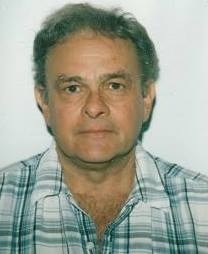
\includegraphics[width=.25\textwidth]{cologero.jpg}
\end{wrapfigure}

Almost two years ago, on the feast day of the Ascension, \textbf{Cologero}, the founder, authority, and genius behind Gornahoor left us behind\footnote{\url{https://www.gpanochfunerals.com/obituary/Charles-Salvo}}. His death was sudden, shocking, and unexpected. For many of us, myself included, Charles was not only a wise voice in the wilderness, but a true sage, a hermetic ``spiritual director'', even a ``spiritual father''. He was the kind of precious and rare teacher who taught his students not only how to understand metaphysics intellectually, but how to actually experience the higher states of being and achieve real metaphysical knowledge.

More than this, Charles taught the transformation of earthly love into spiritual Love, the kind of Love can fuel the rapid and almost vertiginous ascent of the Lover through the Alchemical Marriage\footnote{\url{https://gornahoor.net/?p=13814}}.

In the \textbf{Fedeli d'Amore}\footnote{\url{https://gornahoor.net/?p=10164}}, novices were under a rule of silence for nine years, after which they would write a poem\footnote{\url{https://gornahoor.net/?p=17046}} in order to be initiated. This was the model Charles followed with those he taught personally.

The style of Charles' teaching was unique, and almost ``martial''. He was not a follower of the modern platitude that ``there are no stupid questions''; holding discussion with him on the matters that concerned us was an exercise in rigor and challenge. Like a fencing master calmly dismantling the tentative, feeble strikes of his pupils, Charles swiftly cut through thoughtless, bombastic, or shallow remarks that lacked real understanding. In a way that was stern, but not hostile, Charles used the edge of his saturnine personality to make you instantly feel your own weakness with just a few choice words, or even a pregnant pause. For me (and my experience is not unique), the many years spent striving to engage him on the highest truths, faltering repeatedly, having my own ignorance and errors laid bare; all of this was a crucible essential to my own growth.

\begin{center}* * *\end{center}

Beyond this inner mission of passing on the Hermetic tradition to individual successors, Charles had an outer mission with Gornahoor: \textbf{to return to the foundations of the Western Tradition and chart a path for its renewal}. Gornahoor's has always maintained that this Western Tradition, the ``religion of the Middle Ages'', is the manifestation of the Primordial Tradition, the same Tradition that manifested in the Vedic civilization and in Ancient Greece. The esoteric core of this tradition is called ``The Church of John\footnote{\url{https://gornahoor.net/?p=16881}}'' and Gornahoor has demonstrated its unbroken (if tumultuous) continuity across centuries.

Charles' vision for a reinvigorated Western Tradition was a glorious one. What Julius Evola doubted, Charles, with Guido de Giorgio, dared to hope for:

\begin{quotex}
A Catholicism that is raised up to the level of a truly universal, unanimous, and perennial tradition where faith can be integrated into a metaphysical realization, the symbol integrated into the path to awakening, the rites and sacraments into acts of power, dogmas into expressions of an absolute and infallible consciousness because it is beyond human and, as such, alive in beings unbound from terrestrial chains through an ascesis, and where the pontificate recovers its primal mediating function --- such a Catholicism could supplant every ``spiritualism'', both present and future.

\flright{\textsc{Julius Evola}, \emph{Mask and Face of Contemporary Spirituality}}
\end{quotex}


\begin{center}* * *\end{center}

\textbf{This work is not completed.} Charles wished for the next generation to carry on his work, and \textbf{there are those of us who are prepared to do so.} In 2025 and beyond, Gornahoor will continue Charles' mission in the following ways:

\begin{itemize}


\item New translations of authors like~\textbf{Luigi Valli}\footnote{\url{https://gornahoor.net/?p=6215}} and~\textbf{Guido de Giorgio}\footnote{\url{https://gornahoor.net/?p=5828}}, beginning with Valli's~\emph{Key to the Divine Comedy} and~\emph{Secret Language of the Fedeli d'Amore}.

\item New articles

\item Expansion to new formats (X, Substack\footnote{\url{https://gornahoorpress.substack.com/}})

\item Compilation, preservation, and republication of Cologero's most important writings
\end{itemize}


\begin{center}* * *\end{center}

In Greek, \emph{kalogeros} means ``beautiful elder'', and originally referred to monks or hermits, men who aged gracefully in wisdom and holiness. Hence ``Cologero'', the form the word took when it was adopted in Sicily, the land of Charles' ancestors. The pseudonym was an exact fit for the man behind it.

\begin{quotex}
\begin{verse}
\textbf{Exegi monumentum aere perennius}\\

\textbf{Regalique situ pyramidum altius,}\\

\textbf{Quod non imber edax, non Aquilo inpotens}\\

\textbf{possit diruere aut innumerabilis}\\

\textbf{annorum series et fuga temporum.}\\
\end{verse}
\flright{\textsc{Horace}, \emph{Odes} III: XXX}
\end{quotex}


\textbf{Requiescat in Pace.}



\flrightit{Posted on 2025-03-30 by Tannheuser}

\begin{center}* * *\end{center}

\begin{footnotesize}
\begin{sffamily}
\texttt{T. Freitas on 2025-03-30 at 06:40 said:}

What a thoughtful message! A very well deserved tribute to C.

\hfill

\texttt{oiar on 2025-03-30 at 10:22 said:}

Are there ways of sponsoring the community he envisioned?

\hfill

\texttt{Emanuel Venator on 2025-03-31 at 13:00 said:}

It's good to see Cologero's work continuing. In a very real sense I owe my life to this blog.

\hfill

\texttt{Daft on 2025-04-02 at 02:01 said:}

Wow, nice tribute. As a longtime reader I never knew the face of the mystery person who was so wise and wild to me.

\hfill

\texttt{Sibylle on 2025-04-02 at 03:17 said:}

„Non omnis moriar, multaque pars mei vitabit Libitinam.``

Thank you very much -- and God bless.

\hfill

\texttt{Aria Veritas on 2025-04-10 at 12:50 said:}

I wanted to understand the Red Work and thought he might help out.

The dreams he talked about in his last few months made us both think he would soon go either literally as he did, or metaphysically (which he may also have done).

I'd stopped emailing him (he knew why) six weeks before I heard he'd he died. He died two weeks after what was to be our final correspondence.

I thought he was being stubborn in not emailing to apologise. It was a stupid game but I kept wondering if he had died because he was openly, psychically ``buzzing'' me to go to Gornahoor but I refused. He was so gloriously, hilariously RUDE! Lmao... I also refused to believe he could have *actually* died, because he was buzzing me so consciously.

Quite the blow.

Nevertheless, Zoroastrianism was the first, and it is that which we ought to investigate along with plasma physics before trying to build another crutch for the limping church because if one can grasp the nature of Fire, sacrifice and the meanings of the Arc, we're in business again as a global culture with a unified doctrine.

The following 8 years are integral -- the bridge is wide open right now.

C answered my deepest, most long-held question, answered in (a series of posts on Selene and) a very specific Guénon chapter in Man and His Becoming.

That my question could even BE answered even by Guénon was extraordinary; Charles knew what I was asking, and thanks to his knowledge/strange love I got The Keys. The question was like a God-given, pre-ordained memory code.

I Realised (pun) what had happened via Sufi poetry he sent by Ibn Arabi. I could hardly believe... but had no choice but to believe in all of it, then figure out the mechanics of it. Electrical engineering and plasma physics have never looked so beautiful and perfect.

He teased/tempted publishing some of my writing on his page like Naida if I agreed with him on certain points, but the plasma physics connection and the dodgy nature of western medicine/church are not things to be compromised.

He was one of the few most valuable people I've ever met.

\hfill

\texttt{Juliano on 2025-04-10 at 14:34 said:}

I'm happy that his work will be continued. This site is a constant companion for many years and in a few interactions Charles helped me a lot. God bless you.

\hfill

\texttt{Petter on 2025-04-15 at 09:51 said:}

Thank you for continuing Cologero's work!

Where can I follow it on Substack and X?

\hfill

\texttt{Zebulon Goertzel on 2025-04-16 at 19:24 said:}

Life ain't the same without you Bro

\hfill

\texttt{Tannheuser on 2025-04-30 at 18:56 said:}

Hi Petter,

Substack is \url{https://gornahoorpress.substack.com/}, and my personal X account is on \url{https://x.com/EndymionMk4} , which I'm using primarily for Gornahoor related info/posts.

\hfill

\texttt{Bill on 2025-05-31 at 23:10 said:}

Have you considered reviewing the works of Silvano Panunzio or Attilio Mordini?

\hfill

\texttt{Tannheuser on 2025-06-04 at 13:17 said:}

I haven't, but it could be worthwhile. Thanks for the suggestion.

\hfill

\texttt{Auld Wat on 2025-07-09 at 10:54 said:}

Glad to here Cologero's work is being continued. I will keep you in my prayers as I pray for him.

\hfill

\texttt{Luka Markovic on 2025-10-08 at 18:14 said:}

Thank you for this tribute. Cologero is missed greatly

\hfill

\texttt{Noctael on 2025-11-04 at 14:24 said:}

It could be very useful to have an index to organize the content

\hfill

\texttt{Jean M.M. Bernard on 2025-11-21 at 08:43 said:}

Beautiful tribute.

I had, regrettably, been out of touch with this site and its mastermind for a while, and did not learn about Cologero's passing away before today. I was compelled to check in here after Cologero seemed to appear to me in a dream this morning, communicating certain things which included giving me some kind of old clock in purple. He said that he loves all of you: emphasis on all.

May Our Lord bless him and keep him in His Sacred Heart.

And may his writings endure and inspire great works for the future spiritualization of Mankind.

\end{sffamily}
\end{footnotesize}

